\documentclass[12pt]{article}
\usepackage{amsmath}
\usepackage{amsfonts}
\usepackage{mathrsfs}
\usepackage{lscape}
\usepackage{listings}
\usepackage{graphicx} % Allows for importing of figures
\usepackage{color} % Allows for fonts to be colored
\usepackage{comment} % Allows for comments to be made
\usepackage{accents} % Allows for accents to be made above and below text
%\usepackage{undertilde} % Allows for under tildes to take place for vectors and tensors
\usepackage[table]{xcolor}
\usepackage{array,ragged2e}
\usepackage{hyperref}
\usepackage{framed} % Allows boxes to encase equations and such
\usepackage{subcaption} % Allows for figures to be side-by-side
\usepackage{float} % Allows for images to not float in the document
\usepackage{booktabs}
%\usepackage[margin=0.75in]{geometry}
\usepackage[final]{pdfpages}
\usepackage{enumitem}
\usepackage[section]{placeins}

%%%%%%%%%%%%%%%%%%%%%%%%%  Function used to generate vectors and tensors %%%%%%%%%
\usepackage{stackengine}
\stackMath
\newcommand\tensor[2][1]{%
	\def\useanchorwidth{T}%
	\ifnum#1>1%
	\stackunder[0pt]{\tensor[\numexpr#1-1\relax]{#2}}{\scriptscriptstyle \sim}%
	\else%
	\stackunder[1pt]{#2}{\scriptscriptstyle \sim}%
	\fi%
}
%%%%%%%%%%%%%%%%%%%

\definecolor{mygrey}{rgb}{0.97,0.98,0.99}
\definecolor{codeblue}{rgb}{.2,0,1}
\definecolor{codered}{rgb}{1,0,0}
\definecolor{codegreen}{rgb}{0.3,0.33,0.12}
\definecolor{codegray}{rgb}{0.5,0.5,0.5}
\definecolor{codepurple}{rgb}{0.55,0.0,0.55}
\definecolor{codecyan}{rgb}{0.0,.4,.4}

\lstdefinestyle{mystyle}{
	backgroundcolor=\color{mygrey},   
	commentstyle=\color{codegreen},
	keywordstyle=\color{codeblue},
	stringstyle=\color{codepurple},
	numberstyle=\tiny\color{codegray},
	basicstyle=\footnotesize,
	breakatwhitespace=false,         
	breaklines=true,                 
	captionpos=b,                    
	keepspaces=true, 
	numbers=left,                    
	numbersep=5pt,                  
	showspaces=false,                
	showstringspaces=false,
	showtabs=false,                  
	tabsize=2
}
\lstset{style=mystyle}

\lstset{language=Matlab,backgroundcolor=\color{mygrey}}
\usepackage{lastpage}
\usepackage{fancyhdr}
\pagestyle{fancy}
%\lhead{\large{Nik Benko, John Callaway, Nick Dorsett, Martin Raming}} 
%\chead{\large{\textbf{ME EN 6960: Lab 1}}}
%\rhead{\today}
\cfoot{[\thepage\ of \pageref{LastPage}]}
\fancyheadoffset{.5cm}
\setlength{\parindent}{0cm}
\usepackage[left=.5in, right=0.50in, top=1.00in,bottom=1.00in]{geometry}
\usepackage{microtype} 
\usepackage{setspace}
\doublespace
%%%%%%%%%%%%%%%%%%%%%%%%%%%%%%%%%%%%%%%%%%%%%%%%%%%%%%%%%%%%%%%%%%%%%%%%%%


\begin{document}
\title{ Analysis of Stress Intensity Factors for Mode I and Mixed Mode with Digital Image Correlation \\ \normalsize{ME EN 6960}}
\author{Nik Benko, John Callaway, Nick Dorsett, Martin Raming}
\maketitle


\begin{abstract} 

\end{abstract}

\section{Introduction} 

\begin{abstract}%Nick 
\end{abstract}

\section{Introduction} %Nick


\section{Methods}

\subsection{Experimental Techniques} 
\subsubsection{Mechanical testing} %John
\subsubsection{Digital Image Correlation} % Martin
DIC is a commonly used optical technique in experimental mechanics to accurately measure full-field displacements, and rotations by capturing a sequence of images of a the surface in question. Using two cameras these measurements can be taken in 3D. If only 2D measurements are needed, as in this experiment, only one camera is needed for imaging the surface.
\\
\\
An initial digital image is taken to be used as the reference image which is done before any significant loading of the specimen occurs. Here it is assumed that displacements, and rotations are nearly zero.  This reference image is then compared to a digital image taken once loading has occurred, also know as the deformed image. In many cases numerous digital images are captured during loading for comparison to create a sequence of displacements and rotations.  For correlation to take place an area of interest with in the images is selected and then divided into square sections known as subsets. Each subset is made up of the same number of pixels.  The subsets are matched from the deformed images to the reference image though a correlation function with in the DIC algorithm. By corresponding each pixel to an actual unit of length deformations and rotations can then be tracked using a DIC algorithm \cite{DIC}.
\\
\\
For the DIC algorithm to be effective each subset must contain enough unique features.  These features are related to contrast or pixel values with in each subset. A high-contrast uniform granular  surface is desired to create such usable features. In practice this is known as a speckle pattern. A usable speckle pattern consists of uniformly dispersed speckles of  random shapes and varying sizes. The size of the speckles needed will depend on the size of the specimen and focusing distances. For example, a small specimen with the camera close will require very small speckles while a larger specimen with the camera backed off requires larger speckles. 

\subsubsection{Theoretical Calculations} %John



\subsection{Procedure} %Martin
The experiment was conducted with a thin rectangular PMAA (acrylic) specimen .  To simulate a crack the specimen was cut with a bandsaw directly in the center to a length of 25.4 mm. This  method was chosen to allow for a blunt crack tip so that premature failure of the specimen would not occur while testing.  One side of the plate was painted  completely white and then speckled using a black aerosol paint.  The black paint was applied in a way that allowed for random speckling with in a size range that would allow for proper DIC measurements.
\\ \\
To extract mode I data the  specimen was placed symmetrically in a three-point bend fixture with in an electronic screw-driven Instron machine. A light load was used to hold the specimen in place while the DIC camera was adjusted.
The DIC setup consisted of one camera with ??mm lens mounted to a tripod.  Two green lights  with flexible attachments were positioned and aligned to provide adequate lighting. Green lights aid to increase contrast in monochromatic imaging. Figure \ref{fig:DIC} With the DIC system in place the aperture to the camera was opened fully and the camera lens was then focused referencing the area around the crack tip. Next the aperture and exposure were adjusted so that focus was maintained while not over exposing any aspect of the image. 
\\
\\
We then took several images to obtain an initial reference and to get an estimate of unwanted noise. From here we incremented the load on the specimen while subsequently taking an image at each increment. Care was taken to record the load as close to the point in time that the image was captured since the specimen would relax at the given displacement thus resulting in a steady decreas in load. Once the threshold of 300N was reached we unloaded the specimen.  For mixed mode load we adjusted the three-point fixture to create asymmetric loading. This was achieved by simply moving one support towards the center.  This lead to a gap of four inches from one support to the center on one side and two inches on the other. Just as before the camera was focused and adjusted fallowing incremental loading with correlated images. Table \ref{tab:data} shows the sequence for each load and the correlated image number for both mode I and mixed mode testing. These images were annualized for displacements using an available commercial software named Vic-2D from correlated solutions. 
\subsection{Error and Uncertainties} %Martin
In general DIC is fairly accurate but does have some error associated with pixel size. Vic-2D reports an error for each image that is analyzed with in the correlation results.  The reported error is a measure of correlation accuracy,  more specifically epipolar projection error \cite{Vic-2D} . Since this error is directly related to speckle pattern and camera settings we achieved a uniform error of 0.006 for all of our results.  This is considered a very low value and indicates are results from the DIC analysis are reliable. Other source of error could arise from time between the pictures taken and time at which the load was recorded. The specimen tended to relax under a constant displacement resulting in a dropping load. To best avoid this type of error we had an one individual tasked with taking an image and verbally notifying another who would then read the resulting load to a third individual who would record the image number and load.   

\section{Results}%Nik

\section{Discussion}%Nik

\section{Conclusion}%Nick

\section{Figures}
% DIC setup
\begin{figure}[H]
	\centering
	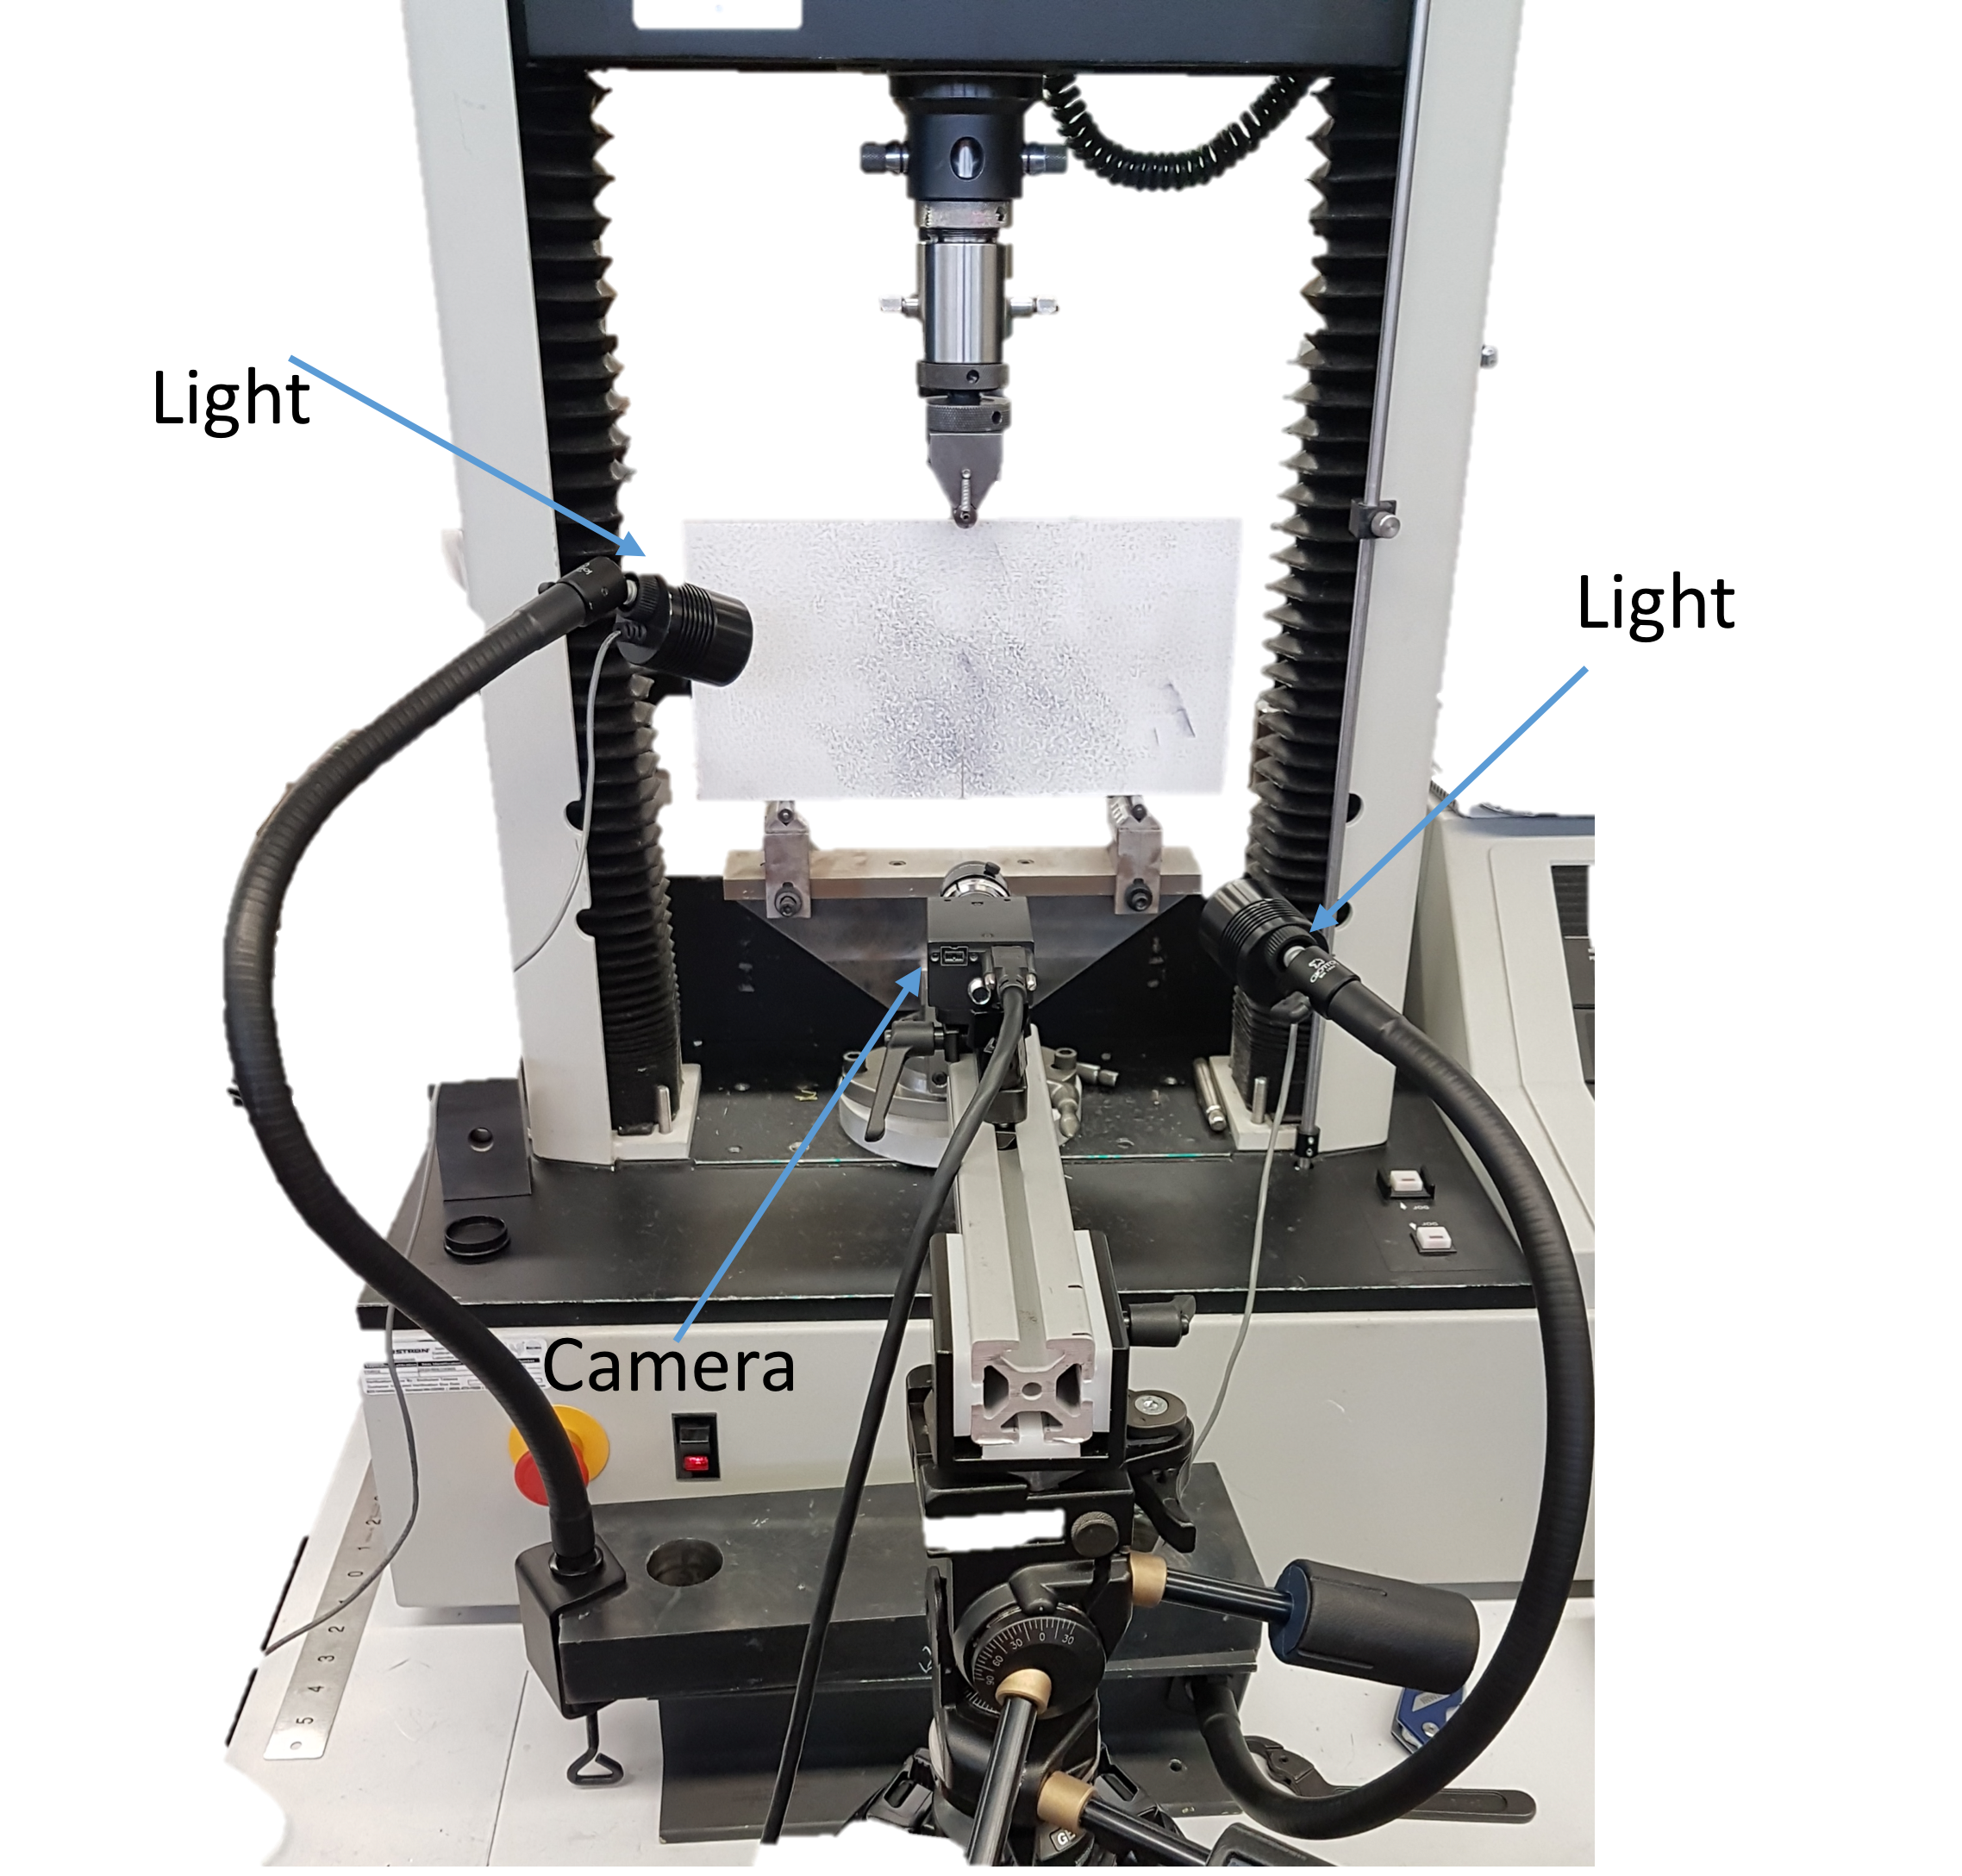
\includegraphics[width=1\textwidth]{DIC Setup.png}
	\caption{The specimen is mounted to the fixture with the DIC system in place, here the camera is fixed to a tripod and two adjustable lights are seen on either side.}
	\label{fig:DIC}
\end{figure}
 
\section{Tables}
Recoded Experimental Data:
\begin{table}[h]\footnotesize
	\centering
	\begin{tabular}{ |l|l|l|l| }
		\hline
		\multicolumn{2}{|c|}{\textbf{Mode I}}&\multicolumn{2}{|c|}{\textbf{Mixed Mode}}\\ \hline
		\textbf{Load [N]} & \textbf{Image Number}&\textbf{Load [N]} & \textbf{Image Number}\\  \hline
		0-5 & 7.784 & 0-4 & 25.58 \\ \hline
		6& 7.784 & 5 & 27.58 \\ \hline
		7 & 93.77 & 6 & 86 \\ \hline
		8 & 215.6 & 7 &191.7 \\ \hline
		9 & 295 & 8 & 324 \\ \hline
		10 & 412 & 9 & 431 \\ \hline
		11 & 489.6 & 10 & 486 \\ \hline
		12 & 587 & 11 & 534.7 \\ \hline
		13 & 745 & 12 & 629.1 \\ \hline
		14 & 834 & 13 & 761.7 \\ \hline
		15 & 899 & 14 & 805.3 \\ \hline
		16 & 952 & 15 & 849.6 \\ \hline
		17 & 1010 & 16 & 896 \\ \hline
		-	& - & 17 & 1000 \\ \hline
		
		
		
	\end{tabular}
	\caption{Loads and associated image number, first few images were used as reference images.}
	\label{tab:data}
\end{table}
% All layups
\
\section{Appendix}

\subsection{equations}


\subsection{Code}

\begin{verbatim}

\end{verbatim}


\bibliographystyle{IEEEtran}
\bibliography{Lab2Bib}
\end{document}